% Viec can lam:
% 1. Conclusion
% 2. Detail for Art-of-the-state 
%     - tf.idf - Okapi
%	  - Pos
%	  - Passage Analyse
% 3. 

\documentclass[12pt, a4paper]{report}
\usepackage[utf8x]{inputenc}
\usepackage{ucs}
\usepackage{amsmath}
\usepackage{amsfonts}
\usepackage{amssymb}
\usepackage{graphicx}
\usepackage{psfrag}
\usepackage{epsfig}
\usepackage[hang,small,bf]{caption} 
\usepackage{amsmath,amssymb}

\usepackage{threeparttable}
\usepackage{colortbl}
\usepackage{slashbox}

\usepackage{algorithmic}
\usepackage{algorithm}

\usepackage{listings} 

\setlength{\captionmargin}{50pt}

\author{Quoc Anh Le}
\title{Master Thesis in Computer Science}

% MARGES
\setlength{\hoffset}{-0.4in} \addtolength{\textwidth}{1.1in}
\setlength{\voffset}{-0.4in} \addtolength{\textheight}{0.2in}


\begin{document}

\begin{center}
\thispagestyle{empty}

\begin{figure}[h]
\centering
\begin{minipage}{5cm}

\includegraphics[width=1\textwidth]{logo-fundp.jpg}
\end{minipage}
\hfill
\begin{minipage}{5cm}

\includegraphics[width=1\textwidth]{Idiap-logo-E.png}
\end{minipage}
\end{figure}

\centering
\vfill

\Huge{\textbf{Automatic true-false question answering in meetings}}\\
\vspace{7mm}
\Large{\textsc{Quoc Anh Le}}\\

\vspace{3mm}
%Master Thesis in Computer Science\\
Master Internship Report \\
\normalsize
\vspace{3mm}
University of Namur \\
Faculty of Computer Science \\
\large

\vfill
\begin{tabular}{l l l}
Supervisor: & Dr. Andrei Popescu-Belis &  (Idiap Research Institute)\\
& & \\
Professor : & Prof. Jean-Paul Leclercq & (University of Namur, FUNDP)\\
\end{tabular}

\vfill
\normalsize
1 August 2008 -  31 January 2009
\end{center}

\newpage

\newpage

\section*{Abstract}

A system on automatic question answering for meeting transcripts is developped using speaker-directed lexical similarity algorithm. The main function of this system is to determine the true and false statement in a pair of two true-false analogous statements. In other words, it answers the following question: which statement is true in a such pair.

Most question answering systems use lexical similarity algorithm in which matched words between a question and a passage is assigned with different score to locate relevant passages most likely to contain the answer. Word score may be calculated thanks to its frequency, its part of speech (PoS) or its relation with neighbour words. In this case, a simple lexical similaritly algorithm is developped in which passage score is not only based on matched words but also on speaker of these words. This technique pays more attention to the features of a meeting transcript.

Its performance is evaluated by answering a set of several hundreds of such pairs. After that, the results are compared with those of human projects using existing meeting browsers. A comparative analysis should indicate whether or not automatic system and human have the same difficulties in answering such questions. The system is also used to mesure the quality of a meeting summary by its scores compared with the score of original transcript, in which the summary is generated by an Automatic Speech Recognition (ASR).


Keywords: Question Answering, Meeting Browser, Passage Retrieval

\newpage
\section*{Acknowledgements}

The first person I would like to express my gratitude is Dr. Andrei Popescu-Belis, my supervisor at the Idiap Research Institute, Switzerland. In fact, he gradually guided me methods in doing research in general and in this project in particular. I recognize that I have learned a lot from him. During 6 months of internship in Idiap, he always encouraged me and this much motivated me andt made me enjoy my work here.

Secondly, I would like to thank all of professors and teachers at the Computer Science Faculty of University of Namur for their interesting and valuable courses, that bring me background knowlege to complete this project. Especially, my special thanks should be sent to Prof. Jean-Paul Leclercq, my co-supervisor. In deed, he is not only my teacher, but also a good friend who gives me useful advices for my works. 

Last but not least, I thank my wife and my son for their understanding and support during my studies.

\newpage
\tableofcontents

\newpage
\listoffigures

\newpage
\listoftables


\newpage

\chapter{Introduction}

In order to search information of past meetings from archived meeting recordings, it is useful to build appropriate tools, generally named meeting browsers. In fact, these browsers are available to locate the information that is searched for. Up to now, there are some general-purpose meeting browser systems that help human users to locate relevant information. Another possibility is to design browsers that locate information automatically, for instance for verification (fact checking) purpose.

In this report, we present a system towards such automatic browser, that verifies fact by determining true and false statement in a pair of two true-false analogous statements. This work builds an assistance that helps human answer BET questions. The performance of this system is evaluated by answering a set of several hundreds of such pairs. Then its results are compared with those of human subjects using existing meeting browsers in order to indicate whether or not automatic anwsering system and humans have the same difficulties in answerinng such questions. 

In fact, this is rather a questions answering system for meeting transcripts. Therefore, like many other question-answering systems, our approach bases on a basic algorithm using lexical similarity. However, we pay more attention to features of a meeting in order to improve the algorithm by assigning different weights to matched words as well as eliminating all words that cause mistakes. For example, meetings are discussed in spoken english, the utterances are direct-speeches related to speaker, while questions are indirect-speeches, etc.

The report contains 6 sections, in which the first is an introduction chapter while the rest of the report provide information in detail. Accordingly, chapter 2 previews some available approaches concerning question- answering that are widely applied in many applications. Then, chapter 3 gives a brief of structure of meeting transcripts and its questions used in this system as well as some profound analysis of data. While chapter 4 provides a description of our approach, chapter 5 presents our experiments and compares the results achieved by our approach and state-of-the-art approaches. Moreover, at the end of the chapter 5, we conduct a comparison and an evaluation: (i) BET results are compared with those of the system in order to show limitations of an automatic answering as well as difficulties for both human and machine; (ii) the system and its data is also used to measure quality of Automatic Speech Recognition (ASR) summaries. Finally, the last chapter is conclusion of the report.



\chapter{State of the art}

The first and the most important step of a question answering system is to retrieve passages considered as the most likely to contain answering information. 

A passage can simply be defined as a sequence of words regardless sentences or paragraphs. Some systems define a passage as a fixed-length block of words. In this system, we use window-based passage whose length depends on the length of question. This means that its length is dynamic. According to Kaszkiel \cite{kaszkiel2001era}, the main advantage of this method is that it is easy to construct irrespective of the text. Therefore, it is suitable for meeting transcripts, using spoken language regardless the order of phrase or text structure. However, the results obtained can be confusing text because phrases and sentences are cut arbitrarily. 

That is why this step plays a decisive role for the system. Its main objective is to show the most relevant passage to a question using a score function or ranking function, that will calculate the score of each passage, based on question words found in current passage. In other words, all passages are ranked according to their similar words to a given question. In fact, passage retrieval is not only used for questions answering system but also for search engine system in which ranking function is used to rank matching documents according to their relevance to a given search query.

The most simple algorithm for this approach is MITRE, proposed by Light\cite{light2002aec}, in which a passage score function counts number of question words found in a passage as score for this passage. That means all words are treated at the same important level. Many questions answering systems use this method as a baseline score to evaluate their performance. The most different thing from method of Ligth to other systems is that each word is assigned by a different score. In other words, they have different ranking function, for instance, using word frequencies (a standard tf.idf model and Okapi BM25, a variant of tf-idf, represents the state-of-the-art as of 2008 and is used in many pratical applications \cite{wiki_ranking_function},..., using part of speech,... . 

All methods above are used to treat matched words as a "bag-of-words" regardless the position of words as well as the distance among words. They are known as traditional approaches. For modern approaches, one algorithm proposed by Cui \cite{cui2005qap} uses dependency relations among words in a sentence. According to Cui, a dependent tree is built thanks to Minipar in which each leaf presents one word and the relation between two words is presented by an arc. Hence, all pairs of words are presented on this tree. Here, the relation is understood as position of two words in a sentence, one may be before or after another. This is possible because an english sentence may be written correctly by changing the position of words, for instance \textit{"Jean wrote a science fiction book = A science fiction book was written by Jean = Jean wrote a book of science fiction = A book of science fiction was written by Jean = Jean wrote a book of fiction of science = A fiction of science book was written by Jean."}. Assuming that we have a sentence \textit{Jean wrote a science fiction book}, thanks to Minipar \cite{minipar}, we can build a tree as follow: \textit{E1 (U E0 (C (root fin) 2 (V wrote (root write) (relation i) 1 (N Jean (root jean) (relation s) (atts (sem (+gname +person)))) E2 (N (root jean) (relation subj) (atts (sem (+gname +person)))) 6 (N book (root book) (relation obj) 3 (Det a (root a) (relation det)) 5 (N fiction (root science fiction) (relation nn) 4 (U science (root science) (relation lex-mod)))))))}. In this tree, the word "write" is the root of tree, this root has two leaves "Jean" and "science", two leaves of "science" are "a" and "fiction", "book" is a leaf of "fiction". This tree describes very well all different forms of the sentence. Take the word "write" as an example, it is always between the word "Jean" and the subphrase "a science finction book" in which the order of words is free for the subphrase. If we have a query, this query will be compared with the tree of sentence passage instead of original sentence in order to give a similarity score.
For the methods using dependency relations, N-gram method is the simplest that considers the relations of consecutive words. One version of n-gram method is proposed by Buscaldi \cite{buscaldi2007ngv}. This method extracts sets of unigrams, bigrams,.., n-grams from the passages and the question in which n is the number of question words. The score of each passage is proportional to the size of the question n-grams found in the passage, which is calculated as the following: the greatest n-gram in the passage is identified and it is assigned a weight equal to sum of all its term weights. Subsequently, smaller n-grams are searched. The sum of all unigram, bigrams,.., n-grams for each passage is compared in order to obtain the best passage.


%Review the state of the art and related work relevant to this project. The idea is to present (critical analysis comes a little bit later) the major ideas in the state of the art right up to, but not including, personal ideas.
%
%This section is organized by idea, and not by author or by publication. For example, if there have been three important main approaches to Passage Retrieval to date, it might organize subsections around these three approaches:


The next step is to extract answer from retrieved passages.... Questions answering system prefers analyzing type of question in order to extract answer. Take questions with "Who" as examples, the system searchs all proper nouns as name of person, wherease for question with "When", the system will search words regarding the time, etc. Another approach is to build some templates of question form before and search these templates in the current passage. 

At this moment, there are not any automatic methods that can effectively estimate the answers of questions answering systems. That is why my system also encouter some difficulties while defining true statement. 


\chapter{Brief of data structure}

\section{Meeting transcripts}
Meeting transcripts used to test the system are seletected from the project Augmented Multi-party Interactions corpus (AMI project) \textit{http://corpus.amiproject.org/}. The meetings are discussed in English, by native or non-native English speakers. 

In a conversational document like meeting, it is sometimes difficult to understand the content of current discuss if we read only a small passage because speakers do not want to repeat subject name. Therefore, this is a difficulty for automatic machine that wants to extract a small passage most likely to contain relevant information concerning the question. Other feature of meeting transcript is that each information is issued generally by one speaker. Thus, for questions ... 

The transcripts are formatted as below:

\small
\begin{verbatim}  
.....
denis : So I don't know if you all received the the a- agenda for this meeting. 
denis : Do you - no? 
mirek : No, I haven't. 
denis : Here it is. 
mirek : Thank you.
agnes : I haven't
denis : So the goal for today are
.....
\end{verbatim}
\normalsize

There are two versions for each transcript, one is made by humans and the other is produced by an ASR (Automatic Speech Recognition). An ASR module was recently developed in the AMIDA project - Augmented Multiparty Interaction with Distant Access \textit{www.amiproject.org}) that this work belongs to. For ASR transcripts, each utterances have a score that presents its important. Thus, some short versions (summaries) of a meeting transcript may be obtained by eliminating utterances of lowest scores. One of the tasks of this system is to mesure the quality of these summaries by replacing the original transcript with one summary and see the results after running same set of questions.

\section{Questions}
Questions are a set of pair of two analogous true-false statements concerning information of the meeting transcript. They are also called \textit{observations of interest} because they are identified as interests to the participants. These questions, used in testing, are produced by a set of observers, who independently watch selected meeting from corpus. The observers have available full recordings from every media source, in parallel, including paper prinouts of the slides accompanying the meeting.

Each observation is stated as a complementary pair of statements, one true and one false. In fact, at the first time, observer creates list of observations that should not be easy to guess without using the meeting information. Then the observations should be simple and concisely stated. For instance:

\begin{verbatim}
...
1
One of the features under consideration is speech recognition.
One of the features under consideration is fingerprint identification.
---------------------------
2
Mirek had not received the agenda for the meeting
Andrei had not received the agenda for the meeting
---------------------------
....
15
Noone has seen the Shawshank redemption
Only two have seen the Shawshank redemption
---------------------------
...
\end{verbatim}
\normalsize

These questions have been used to evaluate the performance of a meeting browser using in the Browser Evaluation Test (BET) \cite{BET}. For this method, human subjects answer questions using a meeting browser and then average performance of this browser is evaluated by speed and precision of answers given by subjects. These BET results will be compared with those of the system later.

In fact, we lost a lot of time to analyse the questions in order to find a relevant algorithm. Firstly, the correct passages for each true statement in the step Passage Retrieval must be done by hand. These passages are treated as reference passages to compare with candidate passage obtained by algorithm in order to verify if the candidate passage is relevant or not. Secondly, these questions are divided into two classes, straightforward questions class and deductive questions class. For deductive questions, it requires a reflexion or a deduction to be able to give good answers that it is difficult to answer even by human. 

For passage retrieval, signals to know that one question is deductive can be described as the following:
	
		- There are not enough matched words: For instance, for the statement "Agnes notes some reasons to not have a display", the only word "display" appears in the correct passage of 70 words while this word also appears in many others passages.
		
		- It requires a good understanding: For example: "Noone have seen the Shawshank redemption", "No one had seen Goodfellas", etc.
		
		- They are expressed in different ways: Take the following statement as an example "According to the manufacturers, the casing has to be made out of wood", in the corresponding passage, it is expressed by the phrase "they've eliminated all of our options except wood". Or the keyword "four" in the question means four words "left", "right", "up", "down" in the corresponding passage, "easy" = "simple", "thump" = "finger", "keypad" = "button", "without" = "not", etc.
		
%Remain questions seem to be straightforward.

What a pity that we were not successful to distinguish deductive questions from straightforward questions by hand. This is really a complex task. The obtained result is very subjective.

Furthermore, when the programme find correct passages, it is still difficult to distinguish one statement from another in a pair  because of analogousness of two statements. They have only one or two different words from each other but these words do not appear in corresponding passages so that they have even the same score after all operations of algorithm.  For instance, for two questions in a pair "Ed commented that they had a product but that cost was going to be a potential problem" and "Ed commented that they had a product and that cost was not going to be a problem". These questions are different from only two words "potential" and "not" and they found the same passages "Ed: It's almost like, Houston, we have a product here. Problem is obviously gonna be cost." How to distinguish one from another statement in this case?

\chapter{Proposed algorithm}

The project proceeds in two phases. The purpose of the first phase is to locate a passage in the meeting transcript which is most likely to contain the answer (i.e, the facts that discriminate between the true and the false statement), using speaker-directed lexical similarity. Then in the second phase, the true and false statement in each pair is answered by analyzing their corresponding passages found in the first phase. From now on, we call a "matched word" as a question word found in current passage. A passage and a search window is equivalent in some cases.

However, a text pre-processing must be done above all in order to normalise the text as well as to reduce the cost of computing.

Below schema describes the process of the system:

\section{Pre-processing}
There are four main steps in this stage.

1) Removing characters not related to words as punctuations: comma, dot, quotation mark, semicolon or exclamation, etc.

2) Converting abbreviated words into full forms: We've becomes We have, I'll becomes I will, etc.

3) Converting numeric forms to text forms: 34 becomes thirty four, 2nd become second, etc.

4) Removing stopwords: For the reason that the questions are indirect-speech statements while the meeting transcript is a direct-speech report, we have to remove words related pronouns: personal pronouns (I, we, you, he, she, it, they, me, him, her, us, them, myself, yourself, himself, herself, itself, ourself, themself, ourselves, themselves, yourselves), possessive pronouns (my, our, your, his, her, its, their, mine, ours, yours, hers, theirs ), demonstrative pronouns (this, that, these, those, which) as a list of stop words. Some prepositions (to, in, at, on, of, about, above, for, by, with, up), conjunctions (and, or, but, nor, so, for, yet) and, articles (a, an, the) are removed because they offer little sematic information and only muddle the signal from the more contenful words according to Hirschman \cite{hirschman1999drr} and in order to reduce cost of computing. \\

Then, both the questions and the transcript are splitted into sequences of words. Stemm is used in order to remove inflectional affixes. This may increase the signal from contentful words. We use the stemmer programme of Porter \cite{porter2001ss}. Lexical meaning is also extended by synonyms and lemmas using WordNet \cite{pasca2001irw}. All words are transformed into lower-case forms. Hence, there are not proper noun or pronoun any more. They will be treated in the same way.


Each question word is considered as a record of 3 fields: Original word, Lemma of word and Stem of Lemma. In fact, lemmatization sometimes returns more than one lemmatized word for original word, hence, this field is established as an array of strings.

\begin{center}
\begin{threeparttable}
\caption{Word splitting for question}
\begin{tabular}{|c|l|l|l|}
\hline  \bf{Position} & \bf{Word} & \bf{Lemma} & \bf{Stem}\\
\hline 1 & Mirek & Mirek & Mirek\\
\hline 2 & had & have & have\\
\hline 3 & not & not & not\\
\hline 4 & received & received receive & receiv\\
\hline ... & & &\\
\hline 
\end{tabular}
\end{threeparttable}
\end{center}

For transcript, each word record has 6 fields in which synonyms are narrowed by part of speech (PoS) produced by QTAG \cite{qtag}. The field "Speaker" indicates name of person who used this word. This field is important to questions that demand a verification "who did what" - a frequent type of questions in experimental data. Position is the original position of word before removing stopwords. This field is used to calculate distance among matched words afterward in the phase 2, true-fase question answering.

\begin{center}
\begin{threeparttable}
\caption{Word splitting for transcript}
\begin{tabular}{|c|l|l|c|l|l|}
%\hline \multicolumn{6}{|c|}{Word splitting} \\
\hline  \bf{Position} & \bf{Word} & \bf{Stem} & \bf{Speaker} & \bf{Synonyms} &\bf{PoS} \\
\hline ... & ... & & & &\\
\hline 14 & received & receiv & deni & have get find obtain ...
 &VBD\\
\hline 18 & agenda & agenda & deni & docket schedul agendum ... & NN\\
\hline 21 & meeting & meet & deni & fill match ensembl contact... & NN\\
\hline ... & ... & & & &\\
\hline 
\end{tabular}
\end{threeparttable}
\end{center}

All data are processed before running main algorithm and stored in RAM in order to speed execution of the programme.

\section{Passage retrieval} 
Its task is detect a relevant passage that contains information of answer.

\begin{figure}[htbp]
\centering
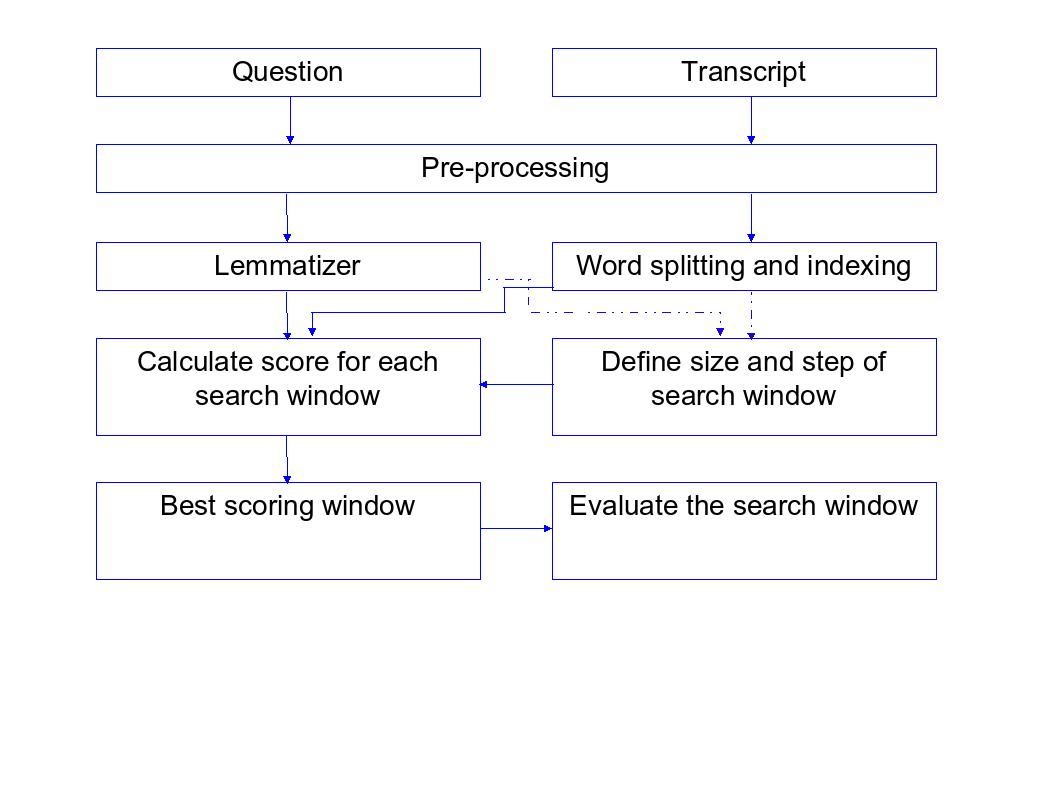
\includegraphics[scale = 0.3]{schema1.jpg}
\caption{Passage Retrieval}\label{fig1}
\end{figure}

\subsection*{Definition of search window size and step}
The programme uses a search window in order to search and calculate score for all passages. It has two parameters: size and step, in which step is a jump of the window. Proposed method for adjustment of the parameters of search window uses size of input question as basic unit, for example, window size = 5 x question size and window step = 2 x question size. This method seems to be suitable to retrieve relevant passage using lexical similarity algorithm because when the length of the question increases, the information that question demands is bigger. Thus, it is necessary to enlarge the size of search window.

\subsection*{Calculation of passage score}

The way calculating passage score determines the effectiveness of a passage retrieval algorithm, but there are no effective methods for all applications. Therefore, to have a good algorithm for each problem, it should better to find some particular features of that problem by analyzing its data.

In this case, each information issued in the meeting is always related to one speaker and most observations of interest (as addressed in the chapter 3) that observers produced have concern with speakers. For this reason, proposed algorithm pays attention to speaker whose name is addressed in question. In detail, passage score increase if the name of a meeting participant is addressed in both question and passage. Then, if matched words are said by this person, score assigned to these matched words will be higher than the other cases.

The algorithm is described as follows:
\begin{algorithm}                      % enter the algorithm environment
\caption{Calculate Passage Score}          % give the algorithm a caption
\begin{algorithmic}                    % enter the algorithmic environment
\REQUIRE Question, Passage, Ngram
\STATE Score = 0

\FOR{i = 1 to length of question} 
	\FOR{j = 1 to length of passage}
	
		\IF{QuesWord[i] is name of a speaker who is present in the passage}
			\STATE Score = Score + Score.Speaker
			\STATE Speaker = Quesword
			\STATE \textbf{break}
		\ENDIF
	
		\STATE Matched = true;
		\FOR{k = 1 to Ngram}
			\IF{Not Matching(QuesWord[i],PasWord[j])}
				\STATE Matched = false
			\ENDIF
		\ENDFOR
		
		\IF{Matched}
			\IF{PasWord[j] is spoken by Speaker}
				\STATE Score = Score + Score.MatchedSpeaker
			\ELSE
				\STATE Score = Score + Score.MatchedWord
			\ENDIF
			\STATE \textbf{break}
		\ENDIF
		
		\IF{QuesWord[i] belongs to synonyms of PasWord[j]}
			\STATE Score = Score + Score.MatchedSynonyms
			\STATE \textbf{break}
		\ENDIF
	\ENDFOR
\ENDFOR

\end{algorithmic}
\end{algorithm}

- The priority order is given to "speaker matching", then "stem matching" and lastly "synonyms matching" in order to bring the highest score for the current passage.

- The frequency of one matched word is not used to increase the score. However, in the case "multiple matching", if one word repeats more than one time in both question and transcript, the score will be calculated as the minimum number of appearance of this word between the question and the transcript.


\newpage

\subsection*{Evaluate retrieved passage}
In order to assess the correctness of a retrieved passage, a reference passage made by hand is used to compare with it. The size of this reference passage is reduced as small as possible but it still contains essential words for answering question. For that reason, even some keywords as name of topic being discussed is not necessary to be included in the reference passage.

The information of the reference passage is the position of its first word and its last word in current transcript. All transcript words are numbered as their position in the transcript by passing name of speakers. For instance:
\small
\begin{verbatim}
.....
denis  :  So I 8 do 9 not 10 know 11 if 12 you 13 all 14 received 
		  the the a- 18 agenda for this 21 meeting. 
denis  :  22 Do 23 you 24 no 
mirek  :  25 No, I 27 have 28 not. 
denis  :  29 Here it is.
mirek  :  32 Thank 33 you.
andrei : I 35 have 36 not 
denis  : So the 39 goal for 41 today are
....
\end{verbatim}
\normalsize

Therefore, for question "Mirek had not received the agenda for the meeting", its relevant passage is (25,28).

If candidate passage and reference passage are overlapped each other, candidate passage is considered correct. The number of overlapped words is fixed as one words or multiple words. If the system is used to help users locate position of answer information, one overlapped will be accepted as well. For experimental system, the number of overlapped words is 1 and the size of retrieved passage is reduced to region which contains matched words instead of size of search window. For example above, the size of search window may be 100 but retrieved passage of highest score by the system will be (14,27) in which 14 is position of the first matched word "received" and 27 is the last matched word "have".

Thus, a function that check correctness of a passage is described as follows:

\begin{algorithm}                      % enter the algorithm environment
\caption{Passage Evaluation}          % give the algorithm a caption
\begin{algorithmic}                    % enter the algorithmic environment

\IF{\\ 
refPas\_pos1 \ensuremath{\leq} catPas\_pos1 \textbf{and} catPas\_pos1  \ensuremath{\leq} refPas\_pos2 \textbf{or} \\
    refPas\_pos1 \ensuremath{\leq} catPas\_pos2 \textbf{and} catPas\_pos2 \ensuremath{\leq} refPas\_pos2 \textbf{or} \\
    catPas\_pos1 \ensuremath{\leq} refPas\_pos1 \textbf{and} refPas\_pos1 \ensuremath{\leq} catPas\_pos2 \textbf{or} \\
    catPas\_pos1 \ensuremath{\leq} refPas\_pos2 \textbf{and} refPas\_pos2 \ensuremath{\leq} catPas\_pos2	\\ }

		\STATE return TRUE
\ELSE
	\STATE return FALSE
\ENDIF

\end{algorithmic}
\end{algorithm}

\newpage

\section{True-false questions answering}
At the first sight, this system seems to be easier than others questions answering system which must analyze the type of question "Who", "when", "how", ... before search answer information in documents. In this case, two questions in a pair are formed as statements and answer is simplely one word "true" or "false" for one question. However, because of analogousness of two questions in a pair, it is really more difficult to distinguish one statement from another by programme.

In this case, we know before that one statement is false in a pair so that it is more probable that passage score of the false statement is less than this of the true statement. That is also main idea of our algorithm for this step. Although of simplicity of this algorithm, experimental results are much better than results by chance.



\begin{algorithm}                      % enter the algorithm environment
\caption{Return true statement}          % give the algorithm a caption
\label{alg1}                           % and a label for \ref{} commands later in the document
\begin{algorithmic}                    % enter the algorithmic environment
\REQUIRE Passage1, Passage2
\STATE score1 = Score of Passage1
\STATE Score2 = Score of Passaag2
\IF{score1 \ensuremath{>} score2}
\STATE return 1
\ELSE [score1 $\equiv$ score2]
	\STATE 	d1 = Distance among matched words between passage1 and question1
	\STATE  d2 = Distance among matched words between passage2 and question2
	\IF{d1 \ensuremath{<} d2}
		\STATE return 1
	\ELSE [d1 $\equiv$ d2]		
		\STATE i = 2;
		\WHILE{Score1 $\equiv$ Score2}		
		\STATE score1 = number of matched i-gram search between passage1 and question1
		\STATE score2 = number of matched i-gram search between passage2 and question2
		\ENDWHILE
		\IF{score1 \ensuremath{>} score2}
			\STATE return 1;
		\ELSE
			\STATE return 2;
		\ENDIF
	\ENDIF
\ENDIF
\end{algorithmic}
\end{algorithm}

\begin{figure}[htbp]
\centering
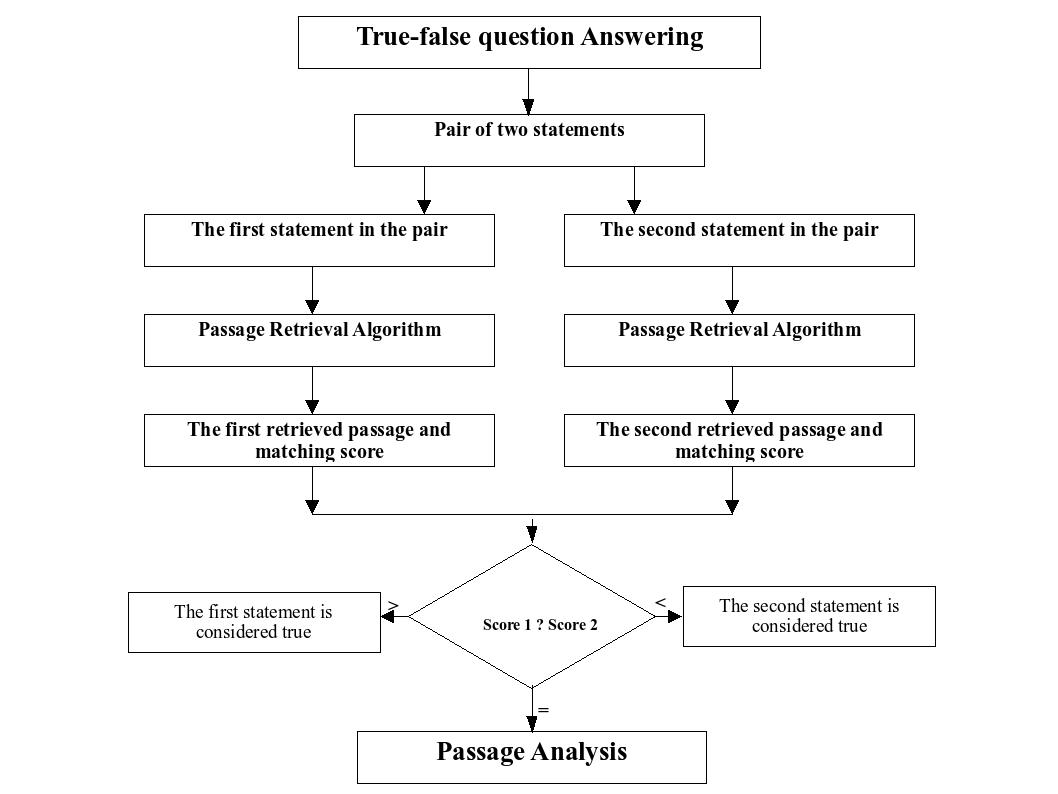
\includegraphics[scale = 0.5]{schema2.jpg}
\caption{True-False Question Answering}\label{fig1}
\end{figure}

\chapter{Experiments and Evaluations}

\section{Data Processing}

The algorithm is experimented on two meetings IB4010 and IS1008c which are collected from the AMI Corpus \textit{http://corpus.amiproject.org}. Both of them are discussed in English, involving four participants, native or non-native English speaker. The first meeting IB4010 lasted 50 minutes in which managers of a movie club discuss to select the next movie to show; meanwhile, in the second one IS1008c, a team discusses the design of a remote control in 26 minutes. There are two versions of transcripts tested, including manual transcripts and automatic transcripts. We have 116 pairs of true-false analogous questions for IB4010 and 50 pairs for IS1008c.

For the manual transcripts, after removing the stopwords, the average length of a question is 8 words, and the length of IB4010 is 4872 words while the length of the original transcript is 9488 words. Meanwhile, the length of IS1008c is 2059 words while the length of the original transcript is 4000 words. The average of question length is 8 words without stopwords.
'

In order to evaluate the performance of the system, we want to divided questions into two classes: straightforward and deductive questions. But as being addressed in the chapter 3, it is difficult. According to our subjective analysis, we find 42 (36.21\%) questions for IB4010 that requires a deduction to answer and only 4(8\%) such questions for IS1008c.  In other words, we have 63.79\% of easy IB4010 questions and 92\% of easy IS1008c questions.
 


\section{System Performance}

The performance of the system must be evaluated by correctness of both passage retrieval module and true-false answering module. The reason for this is that the true-false answering module can even give correct answer but we do not know if this answer bases on relevant information (true passages) or not. However, a relevant passage neither can assure success of a correct answer.


As the belowing, we give some statistics of each step of algorithm. These statistics are very important to understand why the score is too low or too high, what goes wrong and how to fix it.


The method K-fold Cross-Validation \cite{kohavi1995scv} is used to estimate the average of score obtained by this algorithm: 


\begin{table}[ht]
\caption{Results for IB4010} % title of Table
\centering % used for centering table
\begin{tabular}{|l| l | l| l|} % centered columns (6 columns)
\hline\hline %inserts double horizontal lines
Algorithm & Passage Retrieval & True-False Answer & time \\ [0.5ex] % inserts table
%heading
\hline % inserts single horizontal line
    \hline Random  & 0.33\% & 50\% &\\
    \hline Baseline score (unigram) & 26.96\% \ensuremath{\pm}14.78\% & 37.39\% \ensuremath{\pm}13.91\% & 1047584 ms\\
    \hline N-grams & 32.17\% \ensuremath{\pm}15.22\% & 43.48\% \ensuremath{\pm}16.87\% & 3915531 ms\\
    \hline N-grams + speaker-directed weight & 54.78\% \ensuremath{\pm}13.91\% & 57.39\% \ensuremath{\pm}6.52\% & 4489637 ms\\ [1ex] % [1ex] adds vertical space    
	\hline Maximal score by subjective analysis & 63,79\% & 63,79\% & \\
\hline %inserts single line
\end{tabular}
\label{table:nonlin} % is used to refer this table in the text
\end{table}

\begin{table}[ht]
\caption{Results for IS1008c} % title of Table
\centering % used for centering table
\begin{tabular}{|l| l | l| l|} % centered columns (6 columns)
\hline\hline %inserts double horizontal lines
Algorithm & Passage Retrieval & True-False Answer  \\ [0.5ex] % inserts table
%heading
\hline % inserts single horizontal line
    \hline Random  & 0.78\% & 50\%&\\
    \hline Baseline score (unigram) & 54\% \ensuremath{\pm}20.74\% &36\% \ensuremath{\pm}20.74\% & 91017 ms\\
    \hline N-gram search & 50\% \ensuremath{\pm}18.71\%& 42\% \ensuremath{\pm}10.95\% & 466490 ms\\
    \hline N-grams + speaker-directed weight & 62\% \ensuremath{\pm}16.43\%& 64\% \ensuremath{\pm}18.17\% & 640663 ms\\ [1ex] % [1ex] adds vertical space
    \hline Maximal score by subjective analysis & 92\% & 92\% & \\
\hline %inserts single line
\end{tabular}
\label{table:nonlin} % is used to refer this table in the text
\end{table}

In which, score of random method is calculated as below:

Total passages = [(transcript size - window size)/window step] + 1

Correct passage = 2*(window size / window step)

Random score = correct passage/(total passages)

\ensuremath{\Rightarrow} IB4010 score = (2*8*7/7) / ([(4872 - 8*7)/7)   = 0.33%

\ensuremath{\Rightarrow} IS1008c score = (2*8*7/7) / ([(2059 - 8*7)/7)   =  0.78%



\section{Parameters Optimization}

The method K-fold Cross-Validation \cite{kohavi1995scv} is applied to optimize the parameters and also to give the average of the best scores. This method is suitable in the case that algorithm have not enough data to test, so it hides a part of data from building a configuration for the algorithm and after that, it uses these hiden data to test the built configuration.  In this case, for each set of data (transcript, questions), the questions are partitioned into 5 subsets: 4 subsets are used as training data to set the most suitable parameters and the remaining subset is used for testing these parameters. In order to be more visual for reader, 5 subsets are signed as notations \textit{a, b, c, d and e}. So we have 5 pairs (training data, test data) as \textit{1-(bcde,a), 2-(acde,b), 3-(abde,c), 4-(abce,d) and 5-(abcd,e)}. 

With the purpose of calculating the average of highest scores, the algorithm repeates on training data for different parameters from (search window size = 1 x L, search window step = 1 x L) to (search window size = 13 x L, search window step = 13 x L) in which L is the size of input question, so that one pair of parameters offerings the highest score on training data will be given to run on test data.  The average of results obtained from running test data may be considered as the average of highest scores for the unknown data in the future.

The parameters are considered good if they are converged from as many training data as possible. The following tables show a more visual illustration:

For IB4010

% footnote

\begin{center}
\begin{threeparttable}
\caption{Parameters Optimization for IB4010}
\begin{tabular}{|>{\bf}c|c|c|c|c|c|c|c|c|c|c|c|c|c|}
\hline \backslashbox{Size*QS}{Step*QS} & \bf{1} & \bf{2} & \bf{3} & \bf{4} & \bf{5} & \bf{6} & \bf{7} & \bf{8} & \bf{9} & \bf{10} & \bf{11} & \bf{12} & \bf{13} \\ 
\hline 1 &  &  &  &  &  &  &  &  &  &  &  &  &  \\ 
\hline 2 &  &  &  &  &  &  &  &  &  &  &  &  &  \\ 
\hline 3 &  &  &  &  &  &  &  &  &  &  &  &  &  \\ 
\hline 4 &  &  &  &  &  &  &  &  &  &  &  &  &  \\ 
\hline 5 &  &  &  &  &  &  &  &  &  &  &  &  &  \\ 
\hline 6 &  &  &  &  &  &  &  &  &  &  &  &  &  \\ 
\hline 7 &  &  &  &  &  &  &  &  &  &  &  &  &  \\ 
\hline 8 & 1 &  &  & 1 &  &  &  &  &  &  &  &  &  \\ 
\hline 9 & 4 & 3 &  &  &  &  &  &  &  &  &  &  &  \\ 
\hline 10 & 4 & 2 &	\multicolumn{1}{>{\columncolor{blue}}c}{5}\tnote{*} &  &  &  &  &  &  &  &  &  &  \\ 
\hline 11 & 3 & 2 & 5 &  &  &  &  &  &  &  &  &  &  \\ 
\hline 12 & 1 &  &  &  &  &  &  &  &  &  &  &  &  \\ 
\hline 13 &  & 1 & 2 &  &  &  &  &  &  &  & 1 &  &  \\ 
\hline 
\end{tabular}
\begin{tablenotes}
\item[*] This position is choosen to test BET Scores later
\end{tablenotes}
\end{threeparttable}
\end{center}


\begin{center}
\begin{threeparttable}
\caption{Parameters Optimization for IS1008c}
%\begin{tabular}{|>{\bf}c|>{\sc}c|}
\begin{tabular}{|>{\bf}c|c|c|c|c|c|c|c|c|c|c|c|c|c|}
\hline \backslashbox{Size*QS}{Step*QS}  & \bf{1} & \bf{2} & \bf{3} & \bf{4} & \bf{5} & \bf{6} & \bf{7} & \bf{8} & \bf{9} & \bf{10} & \bf{11} & \bf{12} & \bf{13} \\ 
\hline 1 &  &  &  &  &  &  &  &  &  &  &  &  &  \\ 
\hline 2 & 1 &  &  &  &  &  &  &  &  &  &  &  &  \\ 
\hline 3 & 1 & 1 & 1 &  &  &  &  &  &  &  &  &  &  \\ 
\hline 4 & \multicolumn{1}{>{\columncolor{blue}}c}{4}\tnote{*} & 1 & 1 & 1 &  &  &  &  &  &  &  &  &  \\ 
\hline 5 &  &  & 1 & 1 &  &  &  &  &  &  &  &  &  \\ 
\hline 6 & 2 & 2 & 3 & 1 & 2 & 1 &  &  &  &  &  &  &  \\ 
\hline 7 & 1 &  & 3 &  & 2 & 1 &  &  &  &  &  &  &  \\ 
\hline 8 &  &  &  &  &  &  &  & 2 &  &  &  &  &  \\ 
\hline 9 & 3 & 1 & 1 & 1 & 1 & 1 &  &  &  &  &  &  &  \\ 
\hline 10 & 2 &   &	1 & 1 & 1 & 1 &  &  &  & 1 &  &  &  \\ 
\hline 11 & 1 & 1 &   &  &   & 1 & 1 &  &  & 1 &  &  &  \\ 
\hline 12 & 5 & 3 & 3 &  & 2 & 4 & 3 &  &  & 1 & 1 &  &  \\ 
\hline 13 & 1 & 2 & 3 &  & 3 &   & 1 &  &  & 1 & 1 &  &  \\ 
\hline 
\end{tabular}
\begin{tablenotes}
\item[*] This position is choosen to test BET Scores later
\end{tablenotes}
\end{threeparttable}
\end{center}


\begin{figure}[h]
\centering
\begin{minipage}{8cm}
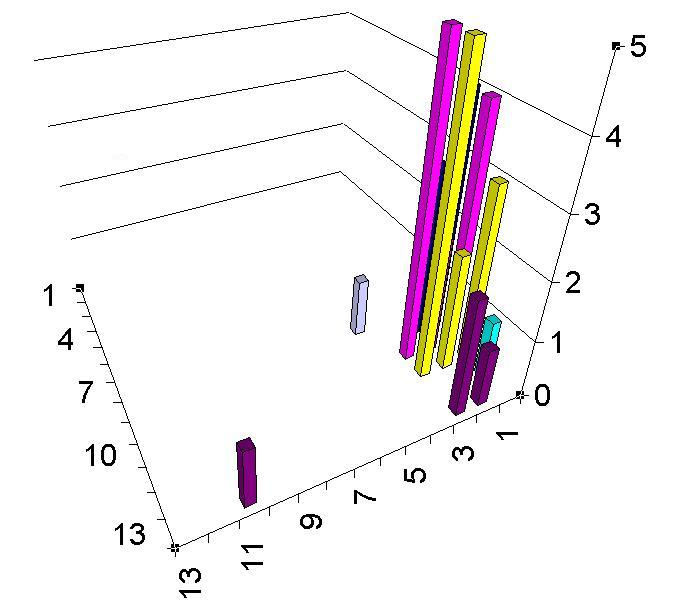
\includegraphics[width=1\textwidth]{Parameters_Optimisation_IB4010.jpg}
%\caption{Parameters Optimisation for IB4010}\label{fig1}
\end{minipage}
\hfill
\begin{minipage}{8cm}
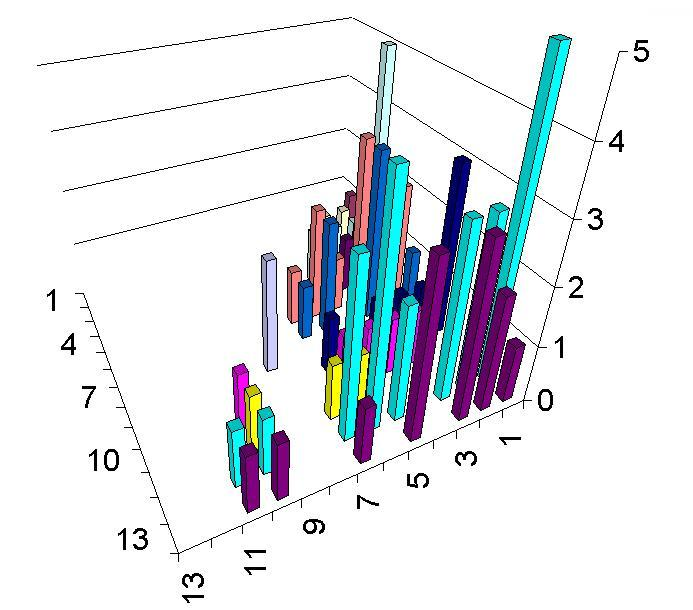
\includegraphics[width=1\textwidth]{Parameters_Optimisation_IS1008c.jpg}
%\caption{Parameters Optimisation for IS1008c}\label{fig1}
\end{minipage}
\caption{Parameters Optimisation for IB4010 (left) and IS1008c (right)}
\end{figure}


In fact, an evident that the more size of search window is large, the higher probability that a passage becomes correct is. When the size of seach window is as equal as the size of transcript, then it certainly contains information of the question. So returned passage is alway true. That is why we rather choose the smallest size of search window that is suitable for most partitions. On the tables, the most suitable parameters for IB4010 is the pair (10,3) and (4,1) for IS1008c. 



\section{Comparing with BET scores by human subjects}
 
We chose two maximal local parameters from previous section (Parameters Optimisation) in order to get results in comparing with BET score by human subjects: (10,3) for IB4010 and (4,1) for IS8001c.

\begin{center}
\begin{threeparttable}
\caption{Questions statistics answered by humans for IB4010 as first meeting}
    \begin{tabular}{ | c | c | c | c | c | c |}
    \hline  \bf{curQid} & \bf{avg time} & \bf{\#subj answd} & \bf{\#correct} & \bf{Precision} & \bf{Speed} \\ 
    \hline 1 & 303,14 & 14			 & 13 & 0,93 & 0,20 \\
	\hline 2 & 105,36 & 14			 & 13 & 0,93 & 0,57 \\
    \hline 3 & 118,14 & 14			 & 10 & 0,71 & 0,51 \\
    \hline 4 & 207,5 & 14			 & 12 & 0,86 & 0,29 \\
    \hline 5 & 64,71 & 14			 & 14 & 1,00 & 0,93 \\
    \hline 6 & 57,79 & 14			 & 13 & 0,93 & 1,04 \\
    \hline 7 & 60,93 & 14			 & 13 & 0,93 & 0,98 \\
    \hline 8 & 129,5 & 14			 & 10 & 0,71 & 0,46\\
    \hline   & 130,88 & & & 0,88 & 0,62 \\
    \hline
    \end{tabular}
\end{threeparttable}

%\textit{http://www.issco.unige.ch/projects/im2/bet/results/stat-questions.php?curMeeting=IB4010&meetingOrder=firstMeeting}
\end{center}

\begin{center}
\begin{threeparttable}
\caption{Questions statistics answered by humans for IB4010 as second meeting}
    \begin{tabular}{ | c | c | c | c | c | c |}
    \hline  \bf{curQid} & \bf{avg time} & \bf{\#subj answd} & \bf{\#correct} & \bf{Precision} & \bf{Speed} \\ 
    \hline 1 & 143 & 14	&10	&0,71&	0,42 \\
	\hline 2 & 66,14 & 14&	14&	1,00&	0,91 \\
    \hline 3 & 89,21 & 14&	14&	1,00&	0,67 \\
    \hline 4 & 206,43 & 14&	12&	0,86&	0,29 \\
    \hline 5 & 37 & 14&	13&	0,93&	1,62 \\
    \hline 6 & 53,21 & 14&	14&	1,00&	1,13 \\
    \hline 7 & 52 & 14&	10&	0,71&	1,15 \\
    \hline 8 & 85,29 & 14&	11&	0,79&	0,70 \\
    \hline   & 91,54 & & & 0,88&	0,86  \\
    \hline
    \end{tabular}
\end{threeparttable}
\end{center}

\begin{center}
\begin{threeparttable}
\caption{Questions statistics answered by the system for IB4010}
    \begin{tabular}{ | c | c | c | c | c | c |}
    \hline  \bf{curQid} & \bf{time} & \bf{\#answd} & \bf{\#correct passage} & \bf{\#correct answd} & \bf{Speed} \\ 
    \hline 1 & 24&1	&0	&0&	2,5 \\
	\hline 2 & 22&1	&1	&1&	2,73 \\
    \hline 3 & 40&1	&1	&1&	1,5 \\
    \hline 4 & 32&1	&1	&1&	1,88 \\
    \hline 5 &16&1	&0	&1&	3,75  \\
    \hline 6 & 17&1	&1	&1&	3,53 \\
    \hline 7 & 24&1	&1	&1&	2,5 \\
    \hline 8 & 19&1	&1	&1&	3,16\\
    \hline   & 194&1	&0,75	&0,88&	2,69 \\
    \hline
    \end{tabular}
\end{threeparttable}
\end{center}

\begin{figure}[h]
\centering
\begin{minipage}{8cm}
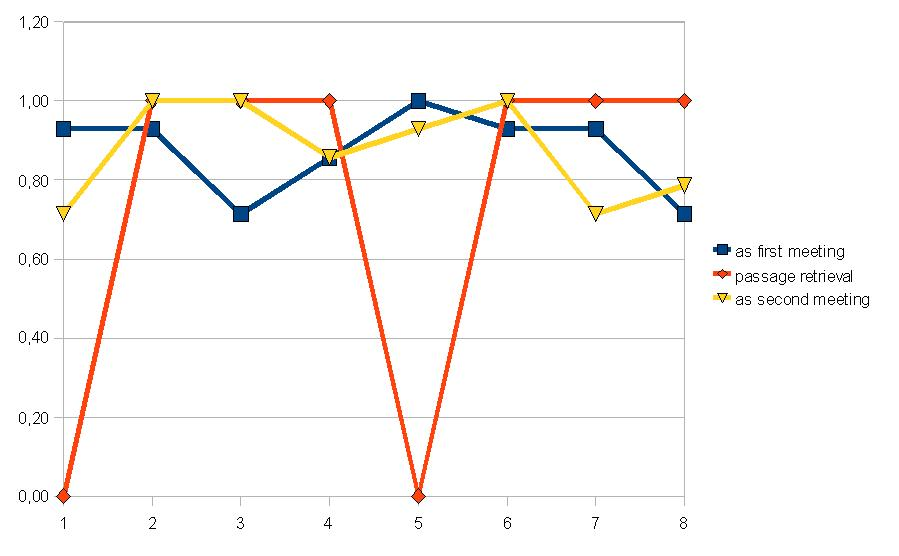
\includegraphics[width=1\textwidth]{BET_results_compararison_IB4010_passage.jpg}
%\caption{Compararison with BET results for IB4010 (Passage retrieval)}
\end{minipage}
\hfill
\begin{minipage}{8cm}
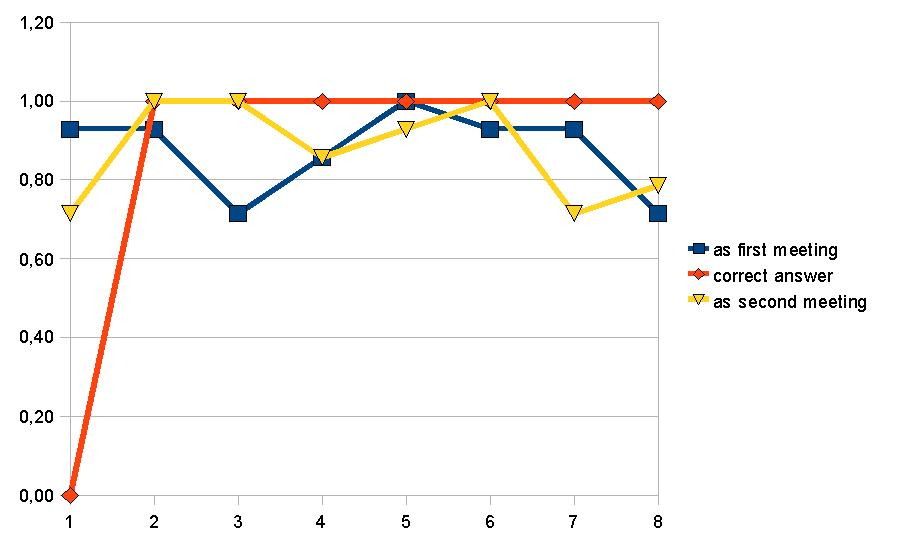
\includegraphics[width=1\textwidth]{BET_results_compararison_IB4010_truefalse.jpg}
%\caption{Compararison with BET results for IB4010 (True-false questions answering)}
\end{minipage}
\caption{Compararison with BET results for IB4010}
\end{figure}

According to precision of answers by human subjects in the table , it is a little bit difficult to answer three questions 1, 7 and 8 while the system gives wrong anwser for two questions 1 and 5. Hence, both human and machine have the same difficulty in answering the question 1. In fact, this question is marked as "Throughout". That means it is neccessary to read all transcripts before answering the question. It is a type of deductive questions. That is why the system could not return correct passage using a small search window. Consequently, its true-false answer is wrong. For the question 5, it requires a deduction for its statement "No one had seen Goodfellas". When all meeting participants said "No" for question "have you seen Goodfellas", it is very easy for human subjects to understand this. But this is really a difficult task for automatic machine. Deduction is a main limitation for all current question-answering systems. Therefore, the system returned a wrong passage.
However, the final true-false answer for question 5 is correct thanks to technique of the algoirthm: corresponding passage score of returned true statement is higher than the other's in the pair.

The question 7 is really easy to be answered by lexical similarity algorithm thanks to many question words found closely in relevant passage. However, some subject still make mistake. This can be explained by the way of comprehensive reading of a human subject. He gives an answer not based on the number of matched words nor density of them but based on comprehension of all text he reads. What a pity that he does not alway understand correctly what othesr express in spoken language, especially in a meeting. In this case, the true statement is "Agnes proposes The Usual Suspects and The Sixth Sense as her movie selections." and the false statement is "Agnes proposes American Beauty and Pulp Fiction as her movie selections.". Then relevant passage should be "Agnes: The Usual Suspects and The Sixth Sense", but Agnes also told about "American Beauty" and "Pulp Fictio" in some other texts. Human subjects located a wrong passage so that they gave a wrong answer.

In temrs of question 8, it should be noted that in this situation "I dislkie Quentins" has the same meaning with "I am not a huge fan of Quentins". This is a deductive question. That is why some human subjects gave a wrong answer. Luckily, there are enough matched words between the true statement and the correct passage, hence, the system gives correct answer.

Meanwgile, the remain questions are really straightforward so that it is easy to answer them for both human and machine. The question 3 seems to be difficult for humans to answer as first meeting but all humans subjects answer it correctly as second meeting.

In this compararison, although there are not many questions but it is enough to show that some deductive questions are not only difficult to be answered by automatic machine but also by human subjects. In many cases, an automatic question-answering system is useful to help human locate relevant passages and then the human analyses these passage to give answer.


\newpage

\begin{center}
\begin{threeparttable}
\caption{Questions statistics answered by humans for IS1008c as first meeting}
    \begin{tabular}{ | c | c | c | c | c | c |}
    \hline  \bf{curQid} & \bf{avg time} & \bf{\#subj answd} & \bf{\#correct} & \bf{Precision} & \bf{Speed} \\ 
    \hline 1 & 410 & 14	& 12	& 0,86 &	0,15\\
	\hline 2 & 298,58 & 12	& 8	& 0,67 &	0,20  \\
    \hline 3 & 78,09 & 11 &	9 &	0,82 &	0,77\\
    \hline 4 & 80,22 &	9	& 8 &	0,89 &	0,75\\
    \hline 5 & 66,38 &	8 &	5 &	0,63 &	0,90\\
    \hline 6 & 44 & 6 &	4 &	0,67 &	1,36 \\
    \hline 7 & 24 & 4 &	4 &	1,00 &	2,50  \\
    \hline 8 & 66 & 3 &	2 &	0,67 &	0,91 \\
    \hline  & 133,41 & & & 0,77	& 0,94  \\
    \hline
    \end{tabular}
\end{threeparttable}
\end{center}

\begin{center}
\begin{threeparttable}
\caption{Questions statistics answered by humans for IS1008c as second meeting}
    \begin{tabular}{ | c | c | c | c | c | c |}
    \hline \bf{curQid} & \bf{avg time} & \bf{\#subj answd} & \bf{\#correct} & \bf{Precision} & \bf{Speed} \\ 
    \hline 1 & 127,36 & 14	& 13 &	0,93	& 0,47 \\
	\hline 2 & 129,5 & 14	& 12 &	0,86 &	0,46  \\
    \hline 3 & 67,5 & 14 &	13	&0,93&	0,89 \\
    \hline 4 & 103,93 & 14&	13 &	0,93&	0,58 \\
    \hline 5 & 63,92 & 13	&9	&0,69&	0,94 \\
    \hline 6 & 62,18 & 11&	8&	0,73&	0,96 \\
    \hline 7 & 48 & 11	&9&	0,82&	1,25  \\
    \hline 8 & 93,55 & 11&	7&	0,64&	0,64  \\
    \hline & 86,99 & & & 0,81 &	0,77 \\
    \hline
    \end{tabular}
\end{threeparttable}
\end{center}



\begin{table}[ht]
\caption{Questions statistics answered by the system for IS1008c} % title of Table
\centering % used for centering table
\begin{tabular}{c c c c c l} % centered columns (6 columns)
\hline\hline %inserts double horizontal lines
curQid & time & \#answd & \#correct passage & \#correct answd & speech  \\ [0.5ex] % inserts table
%heading
\hline % inserts single horizontal line
    1 & 13 & 1 & 1 & 1 & 4,62\\
	2 & 45  & 1 &	1 &	1	& 1,33 \\
     3 & 15 &	1& 1 &	1	& 4 \\
     4 & 16 & 1&	1 &	1&	3,75 \\
     5 & 20 &1&	1 &	0&	3  \\
     6 & 10 &1&	0	&0&	6  \\
     7 & 11 &1&	1&	0	&5,45 \\
    8 & 11 &1&	0&	1&	5,45\\
    Average   & 17,63 &  & 0,75 & 0,63 & 4,2\\ [1ex] % [1ex] adds vertical space
\hline %inserts single line
\end{tabular}
\label{table:nonlin} % is used to refer this table in the text
\end{table}

\begin{figure}[h]
\centering
\begin{minipage}{7cm}
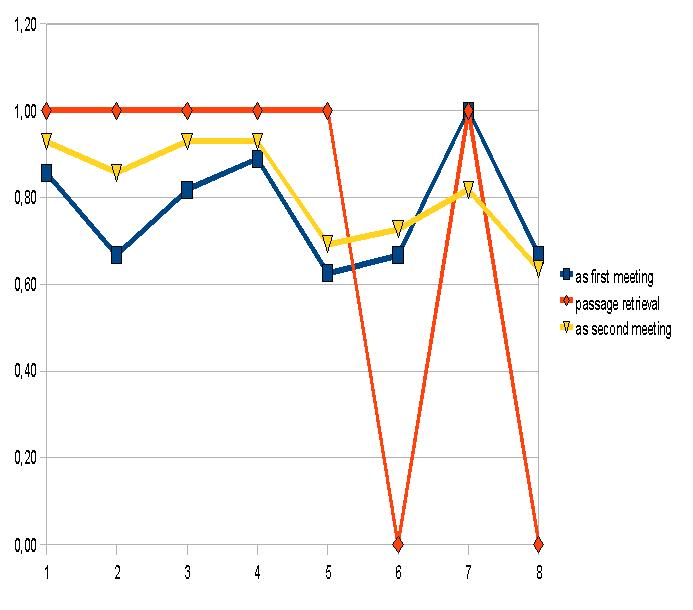
\includegraphics[width=1\textwidth]{BET_results_compararison_IS1008c_passage.jpg}
%\caption{Compararison with BET results for IS1008c (Passage retrieval)}
\end{minipage}
\hfill
\begin{minipage}{7cm}
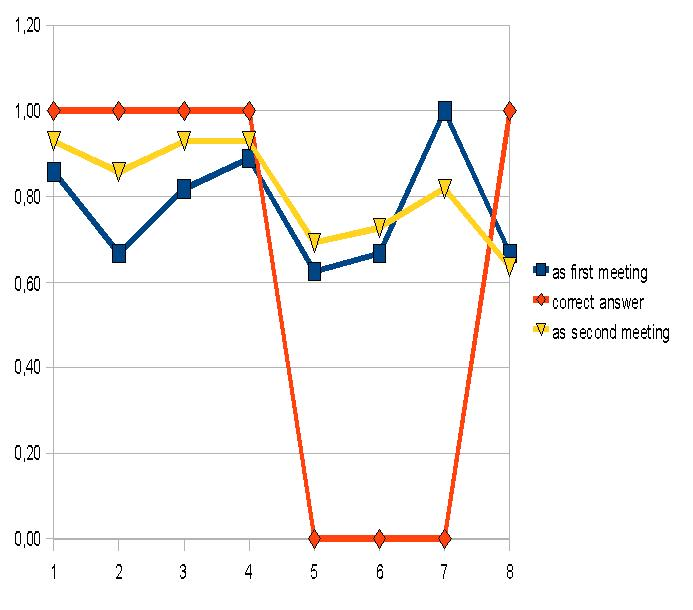
\includegraphics[width=1\textwidth]{BET_results_compararison_IS1008c_truefalse.jpg}
%\caption{Compararison with BET results for IS1008c (True-false questions answering}
\end{minipage}
\caption{Compararison with BET results for IS1008c}
\end{figure}

Concerning BET results compararison for IS1008c, five questions numbered 2, 5, 6, 7 and 8 are a bit more difficult for human to answer than the others, while machine have problem with four questions as the 5th, 6th, 7th and 8th. At the first sight, the results seem to be good that both human and machine encounter the same difficulties in answering such four questions as 5, 6, 7, 8. However, only two questions cause the same difficulty for both of them: question numbered 6 and 8, known as deductive questions, because in order to answer these questions, it requires a good comprehensive reading. Dealing with the statement no. 6, which is "Agnes notes some reasons to not have a display", Agnes showed a list of reasons in the transcript but there is no matched words between the statement and relevant passage except only one word "display". This is similar with the question 8. Although in the second phase, the machine gives correct answer, we can not believe in its reasonableness when it can not determine relevant passage. For human, the results are at very low level for both statistics,using as the first meeting and as second meeting.
This once again confirms that deductive questions are not only difficult for all question-answering systems but also for the human.

In some particular cases, the machine is better than the human when the algorithm treats all words in the same way. For example, keywords in the question 5 are expressed in different ways between the question and relevant passage, "Agnes express her opinon that ..." and "Agne: I think ..." but the same way for words of less importance. That is why the machine gives correct answer while some human subjects make mistake. Unluckily, the machine could not distinguish the true statement from the other in the phase 2. Hence, final answer of machine is not correct. This is the same problem for the question 7 in which the sentence "Problem is obviously gonna be cost" in correct passage must be understood as the meaning of " ... that cost was going to be a potential problem" in the question. From this results, we can draw out a conclusion that the machine is rather better in helping human subjects find relevant passages than in giving correct answer.

In terms the question 2, two statements have one word of difference: "Christine is considering ..." and "Ed is considering ...". This is a typical pair in set of BET questions. By analyzing experimetal results, we find that the machine does not make any mistake to retrieve relevant passage for true statement in such cases. It is thanks to our speaker-directed algorithm.  Then, the machine have shown his advance compared with human in answering such type of questions.







\section{Experiment on ASR summaries}

This section aims at mesuring the quality of a summary generated automatically by its scores.

\begin{center}
\begin{threeparttable}
\caption{Experimental results on ASR summaries for IB4010}
    \begin{tabular}{ | l | l | l | l | l |}
    \hline IB4010 (116 pairs) & length & Passage Retrieval & True-False Answer & time \\ 
    \hline Manual transcript& 4872 & 54.78\% \ensuremath{\pm}13.91\% & 57.39\% \ensuremath{\pm}6.52\% & 4489637 ms\\
	\hline ASR (rank\ensuremath{\geq0.00)}& 4625 & 46.09\% \ensuremath{\pm}12.90\% & 52.17\% \ensuremath{\pm}9.22\% & 5197290 ms \\
    \hline ASR (rank\ensuremath{\geq0.05)}& 3925 & 33.91\% \ensuremath{\pm}9.91\% & 53.04\% \ensuremath{\pm}7.14\% & 3688766 ms \\
    \hline ASR (rank\ensuremath{\geq0.10)}& 3419 & 25.22\% \ensuremath{\pm}12.82\% & 53.04\% \ensuremath{\pm}11.25\% & 4612884 ms \\
    \hline ASR (rank\ensuremath{\geq0.15)}& 3018 & 24.35\% \ensuremath{\pm}7.28\% & 53.04\% \ensuremath{\pm}10.38\% & 3635909 ms\\
    \hline ..............& & & \\
    \hline ASR (rank\ensuremath{\geq0.50)}& 1653 & 13.91\% \ensuremath{\pm}14.87\% & 49.57\% \ensuremath{\pm}9.53\% & 4421315 ms\\
    \hline
    \end{tabular}
\end{threeparttable}
\end{center}


\begin{center}
\begin{threeparttable}
\caption{Experimental results on ASR summaries for  IS1008c}
    \begin{tabular}{ | l | l | l | l | l |}
    \hline  IS1008c (50 pairs) & length & Passage Retrieval & True-False Answer & time \\ 
    \hline Manual transcript& 2059 & 62\% \ensuremath{\pm}16.43\%& 64\% \ensuremath{\pm}18.17\% & 640663 ms\\
	\hline ASR( rank\ensuremath{\geq0.00)}& 1957 & 60\% \ensuremath{\pm}33.62\%& 56\% \ensuremath{\pm}19.49\% & 757834 ms\\
    \hline ASR (rank\ensuremath{\geq0.05)}& 1663 & 70\% \ensuremath{\pm}23.45\%& 54\% \ensuremath{\pm}20.74\% & 869597 ms\\
    \hline ASR (rank\ensuremath{\geq0.10)}& 1457 & 50\% \ensuremath{\pm}15.81\%& 58\% \ensuremath{\pm}8.37\% & 795420 ms\\
    \hline ASR (rank\ensuremath{\geq0.15)}& 1247 & 56\% \ensuremath{\pm}18.17\%& 56\% \ensuremath{\pm}15.17\% & 551357 ms\\
    \hline ..............& & & \\
    \hline ASR (rank\ensuremath{\geq0.50)}& 749 & 20\% \ensuremath{\pm}16.43\%& 64\% \ensuremath{\pm}29.50\% & 410173 ms\\
    \hline
    \end{tabular}
\end{threeparttable}
\end{center}

It seems that the results for IB4010 is more stable than those of IS1008c because the size of IB4010 and its number of questions are two times higher than IS1008c's. However, for both transcrips, they have the same facts:

- The more the length of transcript reduces, the less the number of correct passages we get. Meanwhile, the number correct true-false answers reduce only a little bit. Because reducing transcript size affects both true and false statement in a pair, the score of both corresponding passages reduces accordingly. According the algorithm, statement whose corresponding passage score is higher is considered true. Then, the results of phase 2 is not much changed. As can be seen in the table of results, when we eliminate utterances of less than score 0.5, we have a summary version of 1653 words = 1/3 lenght of original transcript. Then, proportion of correct passages is only 13\% but the proportion of correct true-false answers is still high 49\%.

- For IB4010, the number of correct answers reduces quickly. Thus, it can be said that eliminated utterances play an important roles. However, for IS1008c, the reduction is not very glossy and not quick, this means that eliminated utterances do not contain good information. In conclusion, the score assigned to utterance automatically by ASR is not good.

- The score distribution by ASR seems to be very good: 400-500 words for each interval (0.00-0.05), (0.05-0.10), (0.10-0.15),...

- The time does not increase nor reduce linearly because pairs of questions that the programme can not distinguish using uni-gram. In fact, it has to use bi-grams, tri-grams,... Therefore, even the length of transcript reduces. Nevertheless, if the programme uses more bi-grams, tri-grams,... the time will increase. As a result, on one hand, execution time depends on transcript length, and on the other hand, it depends on the difficulty of questions related to current transcript.

- In terms of original ASR transcripts, they are producted very well by ASR if we compare their scores and their execution time with those of manual transcripts. Moreover, their length is not different from manual transcript's length. 

To conclude: (i) firstly, in this case (for our algorithm), the score of true-false question answering is not suitable to judge the performance of an automatic summary machine; (ii) secondly, for this particular summaries, the ASR is not good to make summaries.



\chapter{Conclusion}
% Recapitulation des axes essentiels du travail, mettant en evidence l'apport original qu'il constitue. Il ne faut jamais introduire d'elements nouveaux dans une conclusion.	
% Tranh su pho truong, chi dan ko hop thoi

\section{Conclusion}

%Conclusions are not a rambling summary of the thesis: they are short, concise statements of the
%inferences that you havemade because of yourwork. It helps to organize these as short numbered
%paragraphs, ordered from most to least important. All conclusions should be directly related to
%the research question stated in Section 4 (Proposed problems).

\section{Summary of contributions}

%The Summary of Contributions will be much sought and carefully read by the examiners. Here
%you list the contributions of new knowledge that your thesis makes. Of course, the thesis itself
%must substantiate any claims made here. There is often some overlap with the Conclusions, but
%that’s okay. Concise numbered paragraphs are again best. Organize from most to least important.

\section{Future Research}

%The Future Research subsection is included so that researchers picking up this work in future
%have the benefit of the ideas that you generated while you were working on the project. Again,
%concise numbered paragraphs are usually best.


\chapter*{Appendix}

%What goes in the appendices? Any material which impedes the smooth development of your
%presentation, but which is important to justify the results of a thesis. Generally it is material
%that is of too nitty-gritty a level of detail for inclusion in the main body of the thesis, but which
%should be available for perusal by the examiners to convince them sufficiently. Examples include
%program listings, immense tables of data, lengthy mathematical proofs or derivations, etc.






\bibliographystyle{plain}	% (uses file "plain.bst")
\bibliography{biblio}		% expects file "myrefs.bib"


\end{document}